\documentclass[border=2pt]{standalone}
\usepackage[T1]{fontenc}
\usepackage{mathptmx}
\usepackage{tikz}
\usetikzlibrary{arrows.meta,positioning,fit,calc,shapes.geometric,backgrounds}
\usepackage{siunitx}
\tikzset{
  >={Stealth[length=1.8mm]},
  blk/.style={draw, thick, minimum height=11mm, text width=16mm, align=center, font=\scriptsize, inner sep=1.5pt, fill=white},
  lab/.style={font=\scriptsize, align=center},
  every picture/.style={line width=0.6pt},
}

\begin{document}
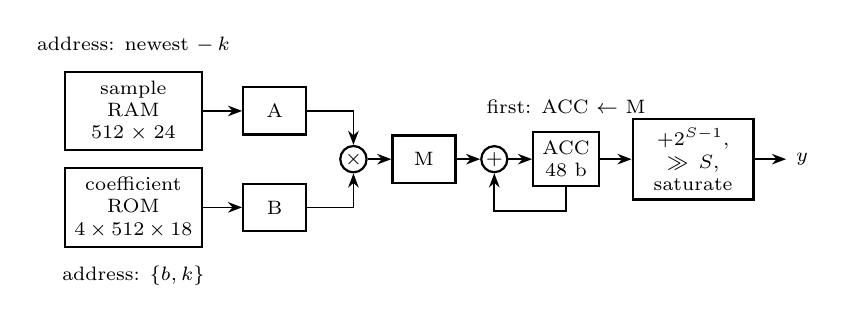
\begin{tikzpicture}[r/.style={draw, thick, minimum width=8mm, minimum height=6mm, font=\scriptsize, align=center},
  m/.style={draw, thick, minimum height=8mm, font=\scriptsize, align=center, text width=15mm}]
\node[m] (ram) {sample RAM\\$512\times24$};
\node[m, below=2mm of ram] (rom) {coefficient ROM\\$4\times512\times18$};
\node[r, right=5mm of ram] (a) {A};
\node[r, right=5mm of rom] (b) {B};
\node[draw, thick, circle, inner sep=0.5pt, font=\scriptsize] (mul) at ($(a)!0.5!(b)+(10mm,0)$) {$\times$};
\node[r, right=3mm of mul] (mr) {M};
\node[draw, thick, circle, inner sep=0.5pt, font=\scriptsize, right=3mm of mr] (add) {$+$};
\node[r, right=3mm of add] (p) {ACC\\48 b};
\node[m, right=4mm of p, text width=13mm] (rs) {$+2^{S-1}$,\\$\gg S$,\\saturate};
\draw[->] (ram) -- (a); \draw[->] (rom) -- (b);
\draw[->] (a) -| (mul); \draw[->] (b) -| (mul);
\draw[->] (mul) -- (mr); \draw[->] (mr) -- (add); \draw[->] (add) -- (p); \draw[->] (p) -- (rs);
\draw[->] (rs.east) -- ++(4mm,0) node[right, font=\scriptsize]{$y$};
\draw[->] (p.south) -- ++(0,-3mm) -| (add.south);
\node[font=\scriptsize, above=1mm of ram] {address: newest $-\,k$};
\node[font=\scriptsize, below=1mm of rom] {address: $\{b, k\}$};
\node[font=\scriptsize, above=1mm of p] {first: ACC $\leftarrow$ M};
\end{tikzpicture}
\end{document}
